\chapter{Results}
This chapter aims to present the results to the reader.
We tested four mechanisms for their utility and privacy, as indicated in the methodology.
For all four mechanisms, we applied a prefix to indicate the number of dimensions on which the mechanism was used.
For example, we named the piecewise mechanism used on 2-dimensional data as "2d-piecewise," even though the underlying method is not different from the original piecewise method.
The results are presented in the following order:
\begin{enumerate}
    \item Research question 1
    \item Research question 2
    \item Influence of the number of dimensions
\end{enumerate}
Research question 3 is already included in the previous two research questions (laplace-optimal-truncated).
\newpage
\section{Research question 1}

% For research question 1 the results are 2-dimensional plotted using a line diagram.
\subsection{Utility}
\subsubsection*{Cluster comparison}
%\todo[inline]{Add plot}
\subsubsection*{Mechanism comparison}
\begin{figure}[H]
    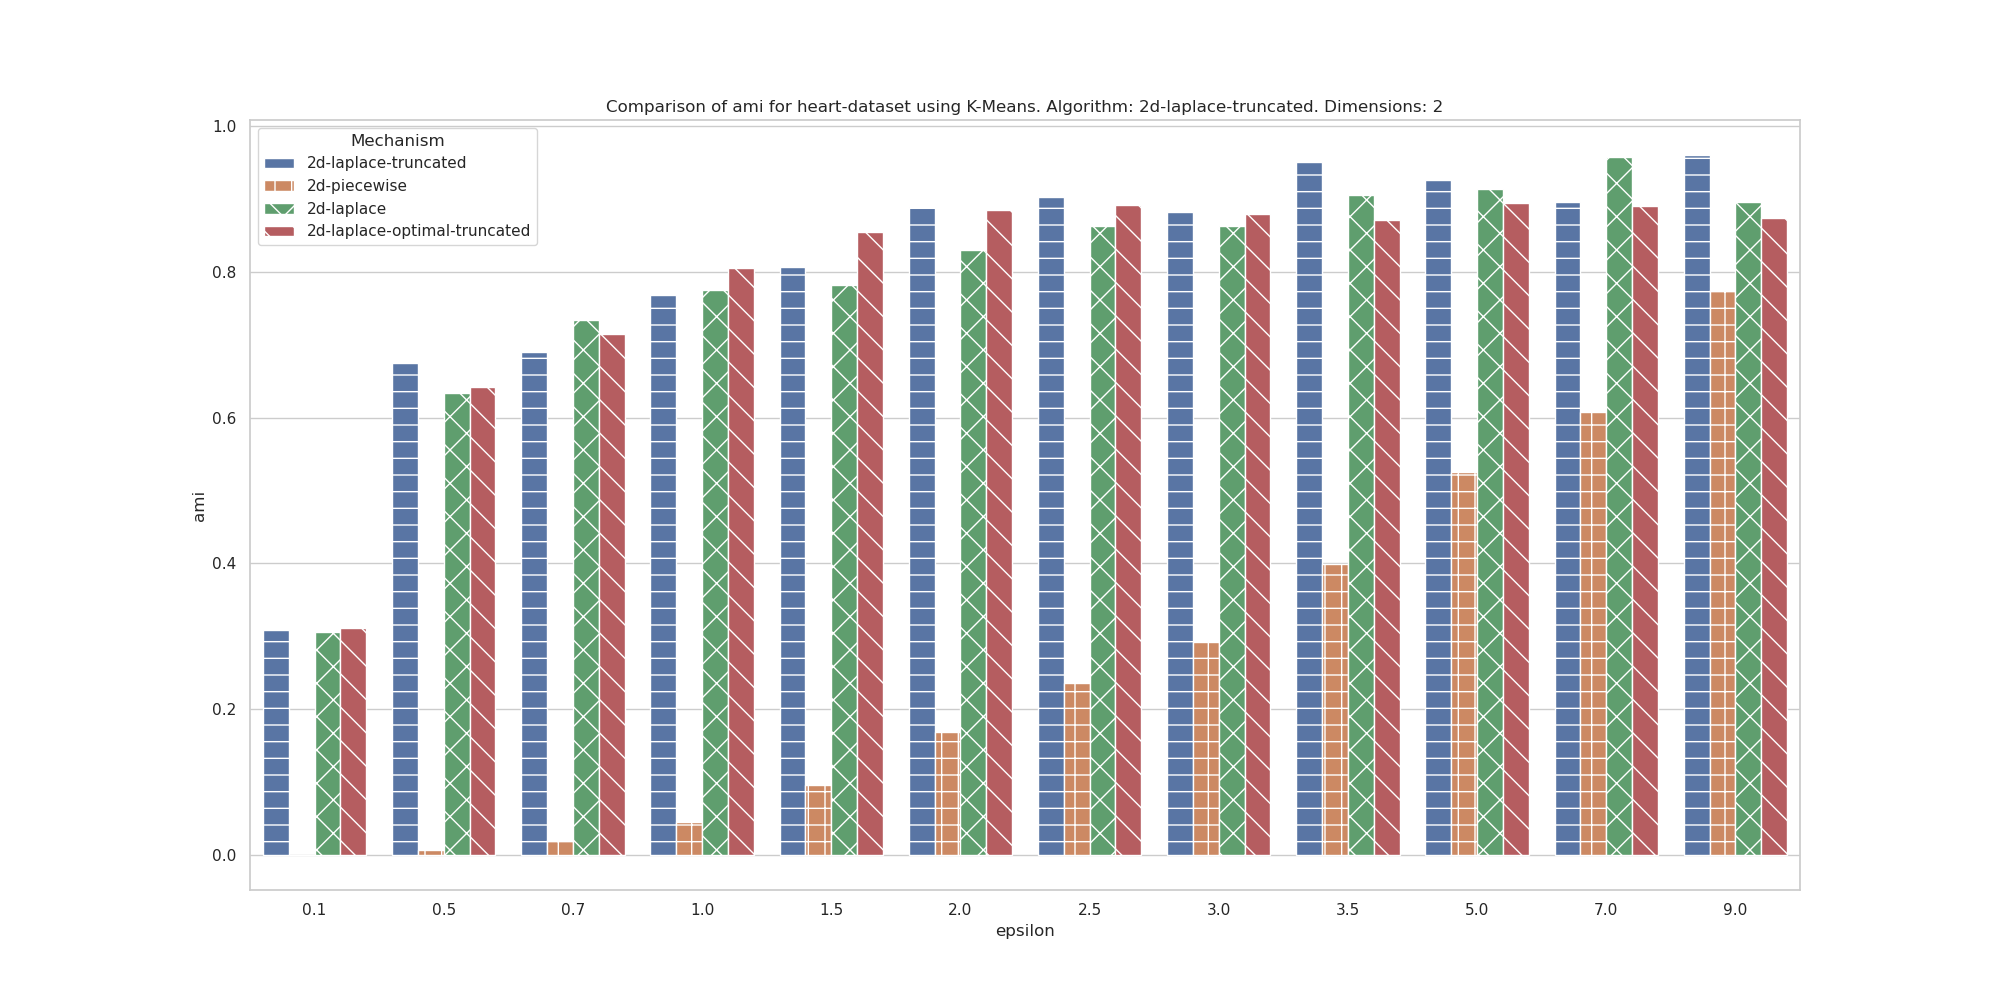
\includegraphics[width=1\textwidth]{Results/RQ1/heart-dataset/ami_heart-dataset_comparison.png}
    \caption{Adjusted Mutual Information comparison for the heart-dataset}
    \label{fig:ami_heart-dataset_comparison_2d}
\end{figure}
\begin{figure}[H]
    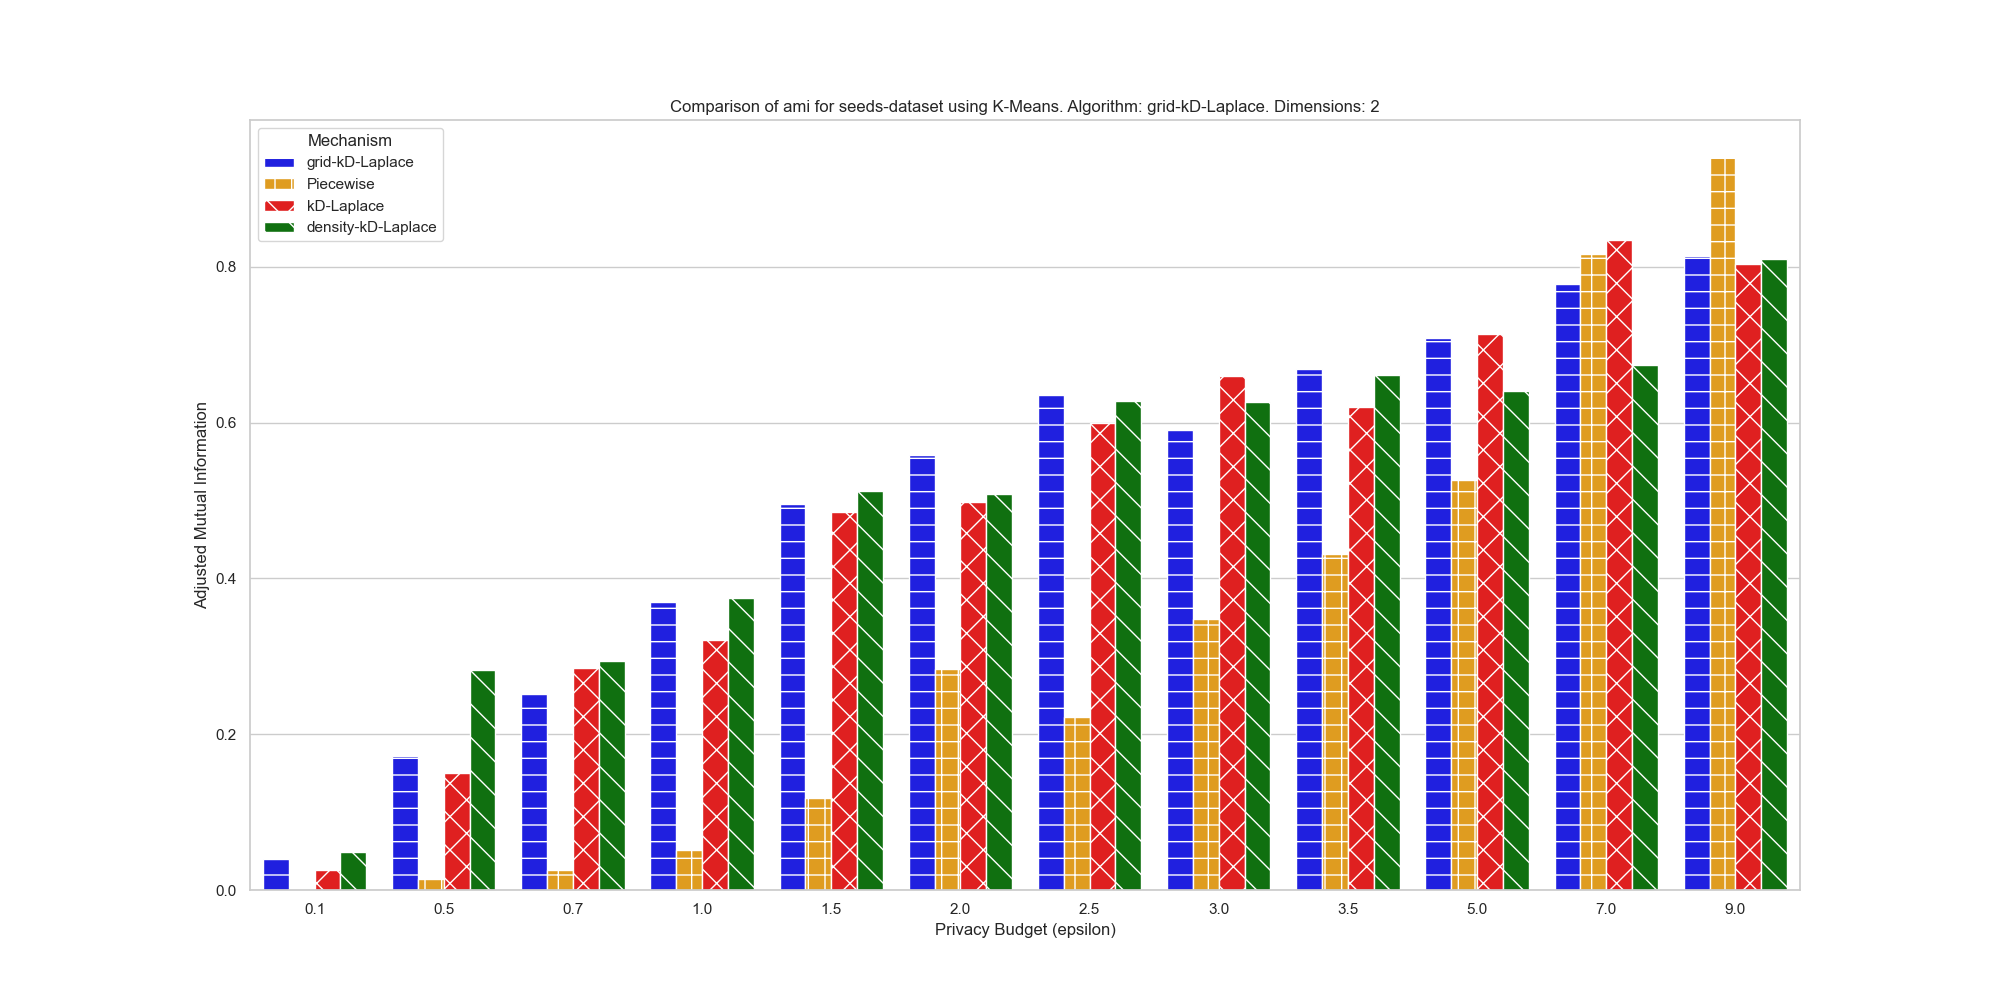
\includegraphics[width=1\textwidth]{Results/RQ1/seeds-dataset/ami_seeds-dataset_comparison.png}
    \caption{Adjusted Mutual Information comparison for the seeds-dataset}
    \label{fig:ami_seeds-dataset_comparison_2d}
\end{figure}
\todo[inline]{Add links to scilliouette plots and other plots}
\subsection{Privacy}
\begin{figure}[H]
    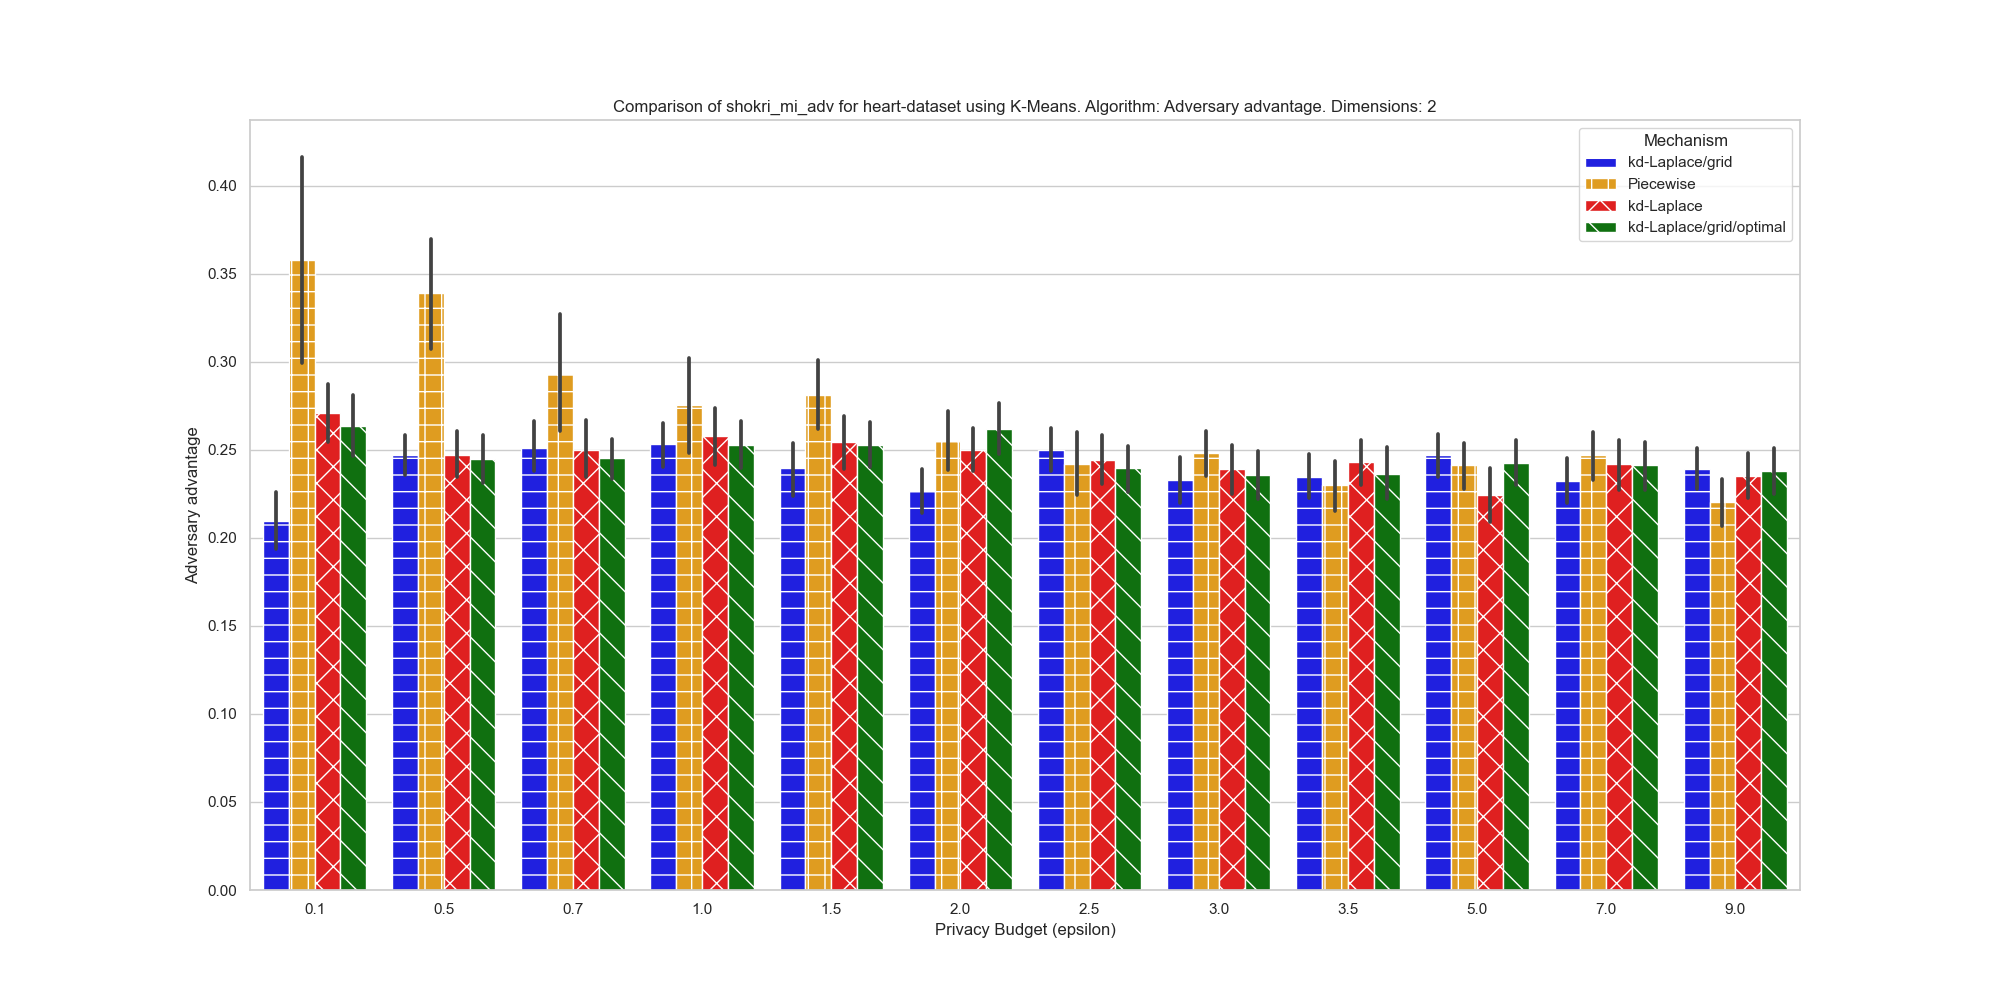
\includegraphics[width=\textwidth]{Results/RQ1/heart-dataset/shokri_mi_adv_heart-dataset_comparison.png}
    \caption{Skokri et al. privacy comparison for the heart-dataset.}
    \label{fig:privacy_heart-dataset_comparison_2d}
\end{figure}
\begin{figure}[H]
    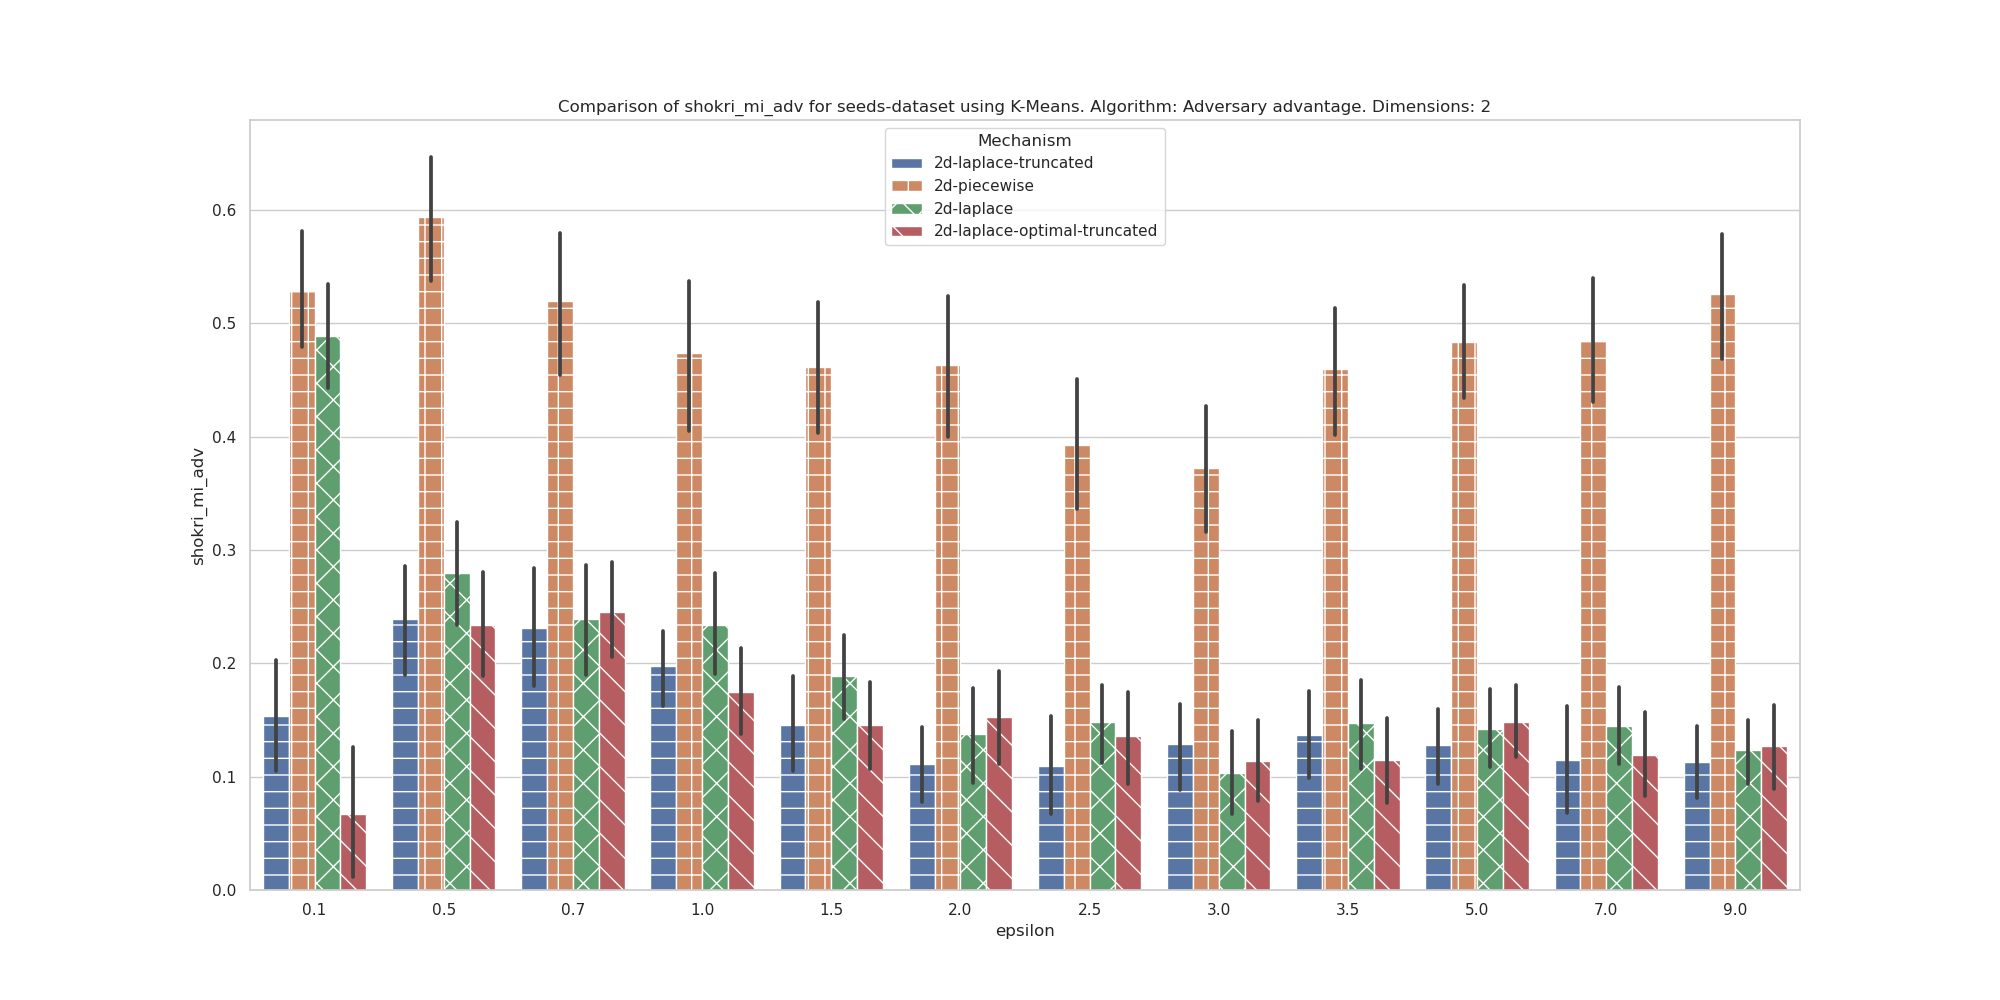
\includegraphics[width=\textwidth]{Results/RQ1/seeds-dataset/shokri_mi_adv_seeds-dataset_comparison.png}
    \caption{Skokri et al. privacy comparison for the seeds-dataset.}
    \label{fig:privacy_seeds-dataset_comparison_2d}
\end{figure}
\begin{figure}[H]
    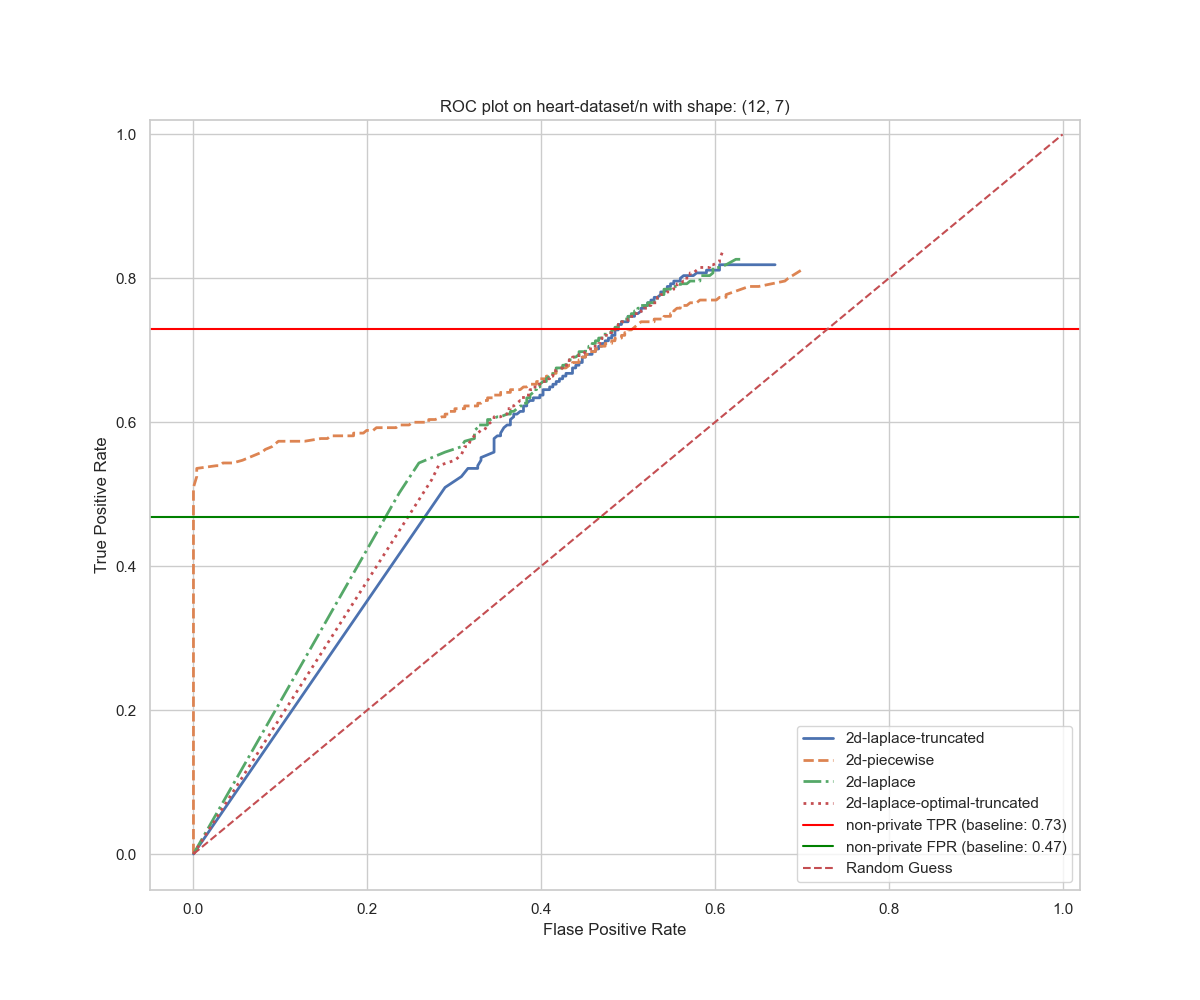
\includegraphics[width=0.8\textwidth]{Results/RQ1/heart-dataset/roc_plot.png}
    \caption{ROC-curve for privacy per privacy mechanism for heart-dataset.}
    \label{fig:privacy_heart-dataset_comparison_2d_roc_plot}
\end{figure}

\begin{figure}[H]
    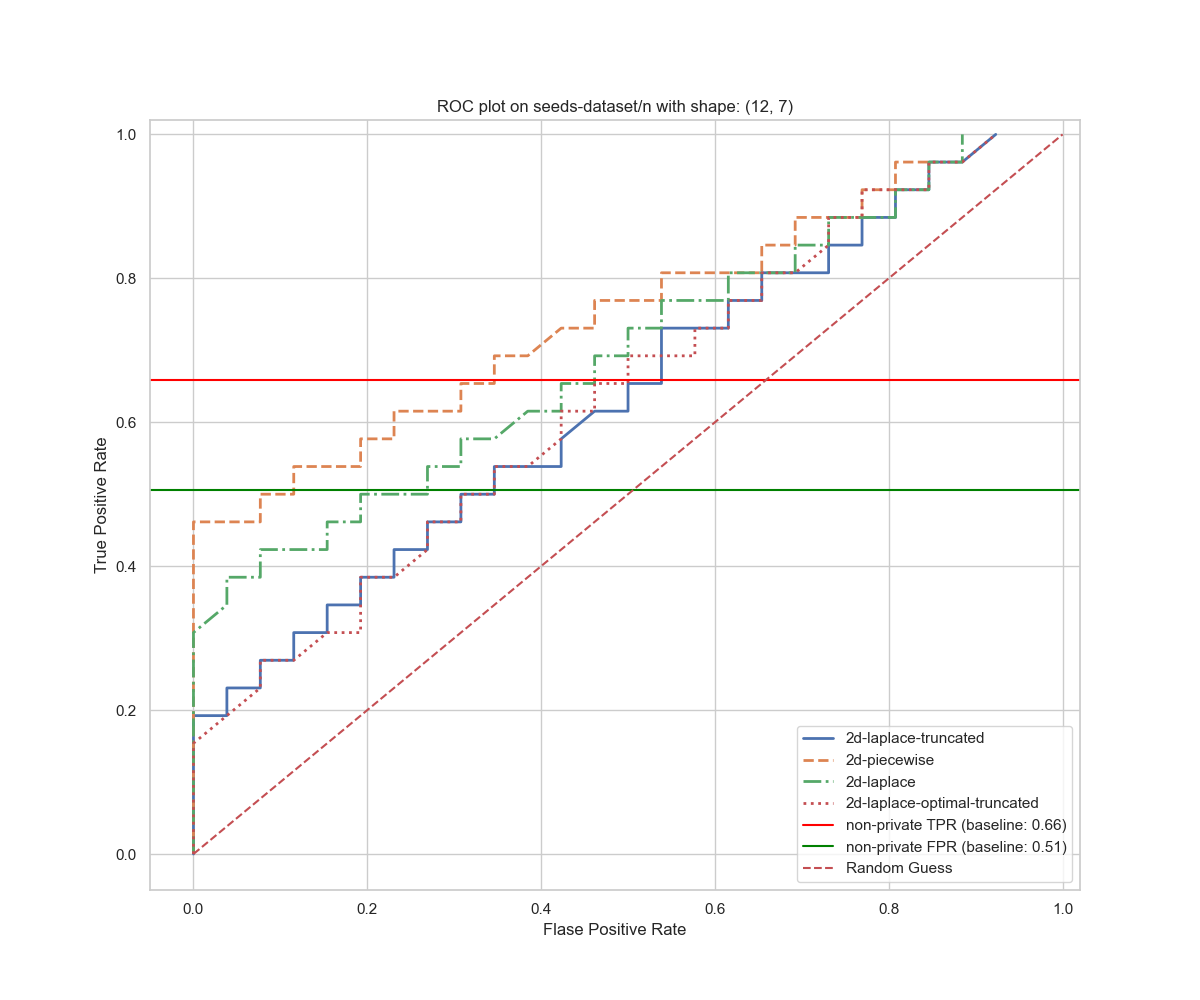
\includegraphics[width=0.8\textwidth]{Results/RQ1/seeds-dataset/roc_plot.png}
    \caption{ROC-curve for privacy per privacy mechanism for seeds-dataset.}
    \label{fig:privacy_seeds-dataset_comparison_2d_roc_plot}
\end{figure}

\newpage
\section{Research question 2}
\subsection{Utility}
\subsubsection*{Cluster comparison}
\todo[inline]{Add plot}
\subsubsection*{Mechanism comparison}
\begin{figure}[H]
    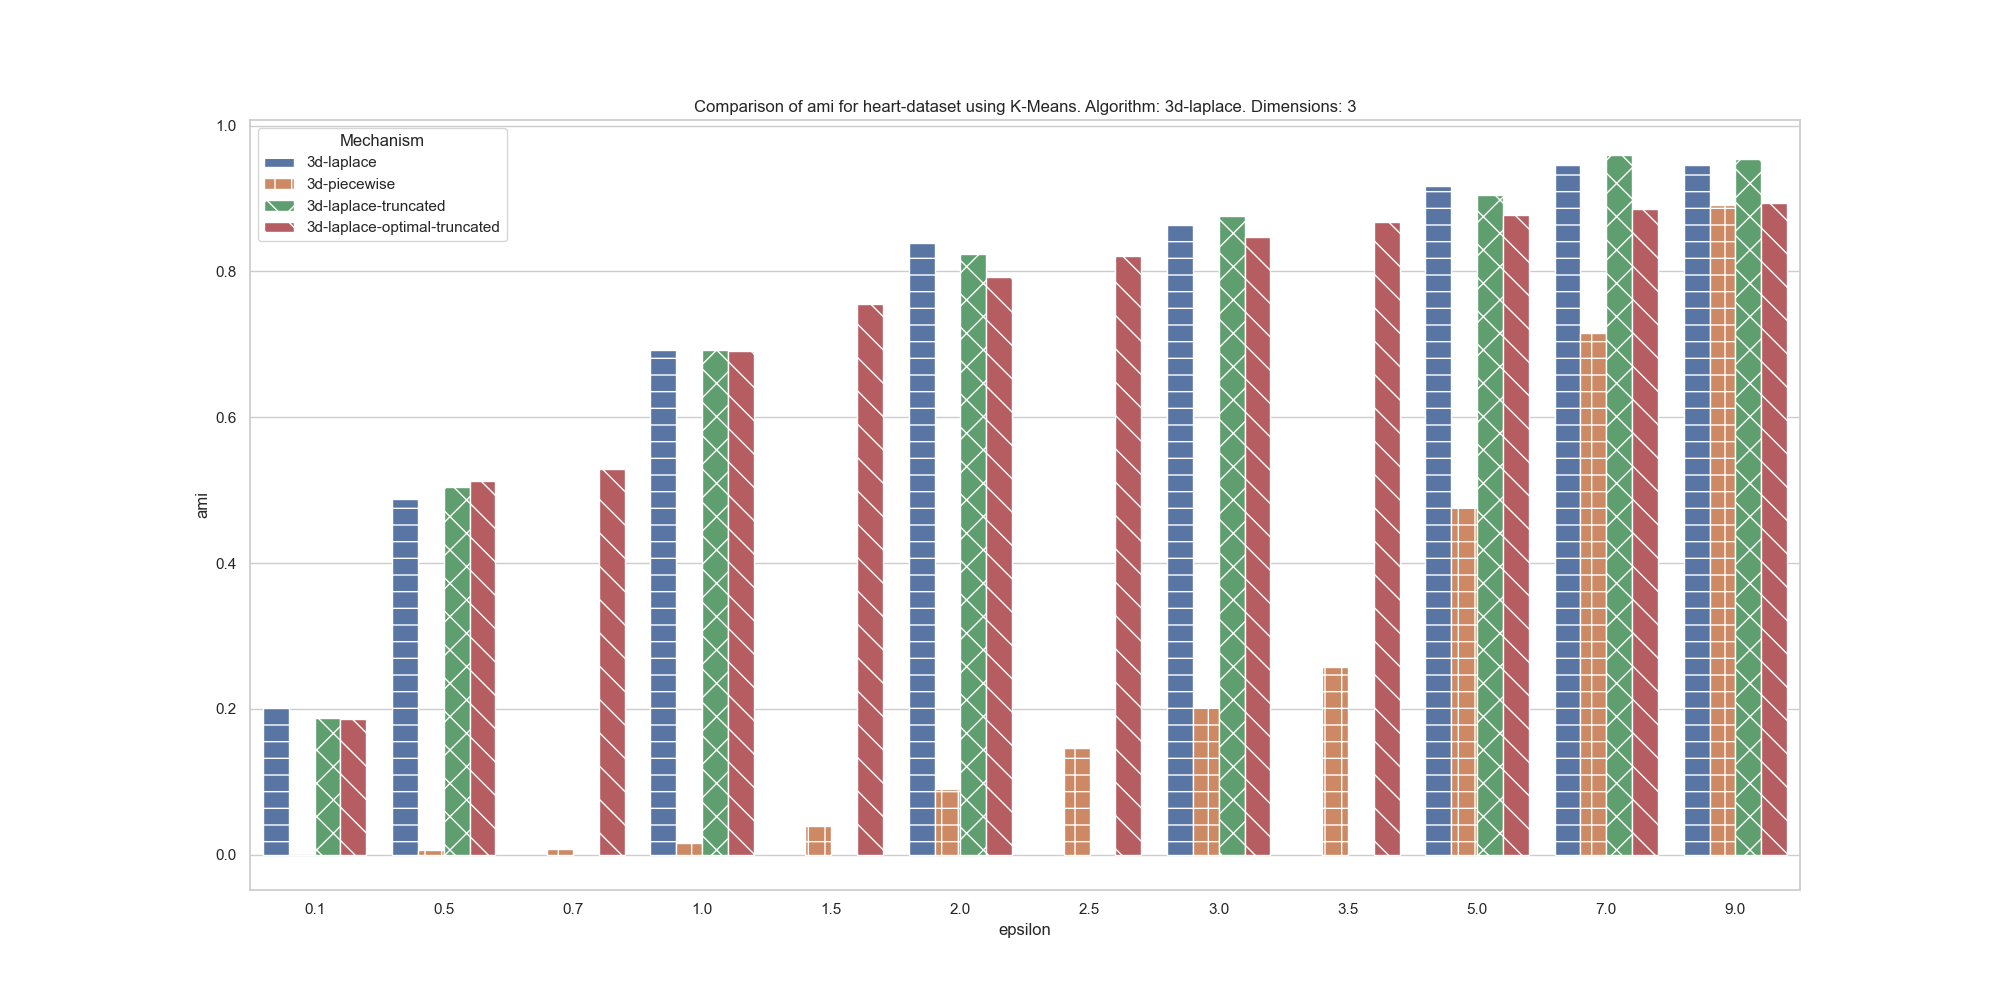
\includegraphics[width=\textwidth]{Results/RQ2/heart-dataset/ami_heart-dataset_comparison.png}
    \caption{Adjusted Mutual Information comparison for the 3-dimensional heart-dataset}
    \label{fig:ami_heart-dataset_comparison_3d}
\end{figure}
\begin{figure}[H]
    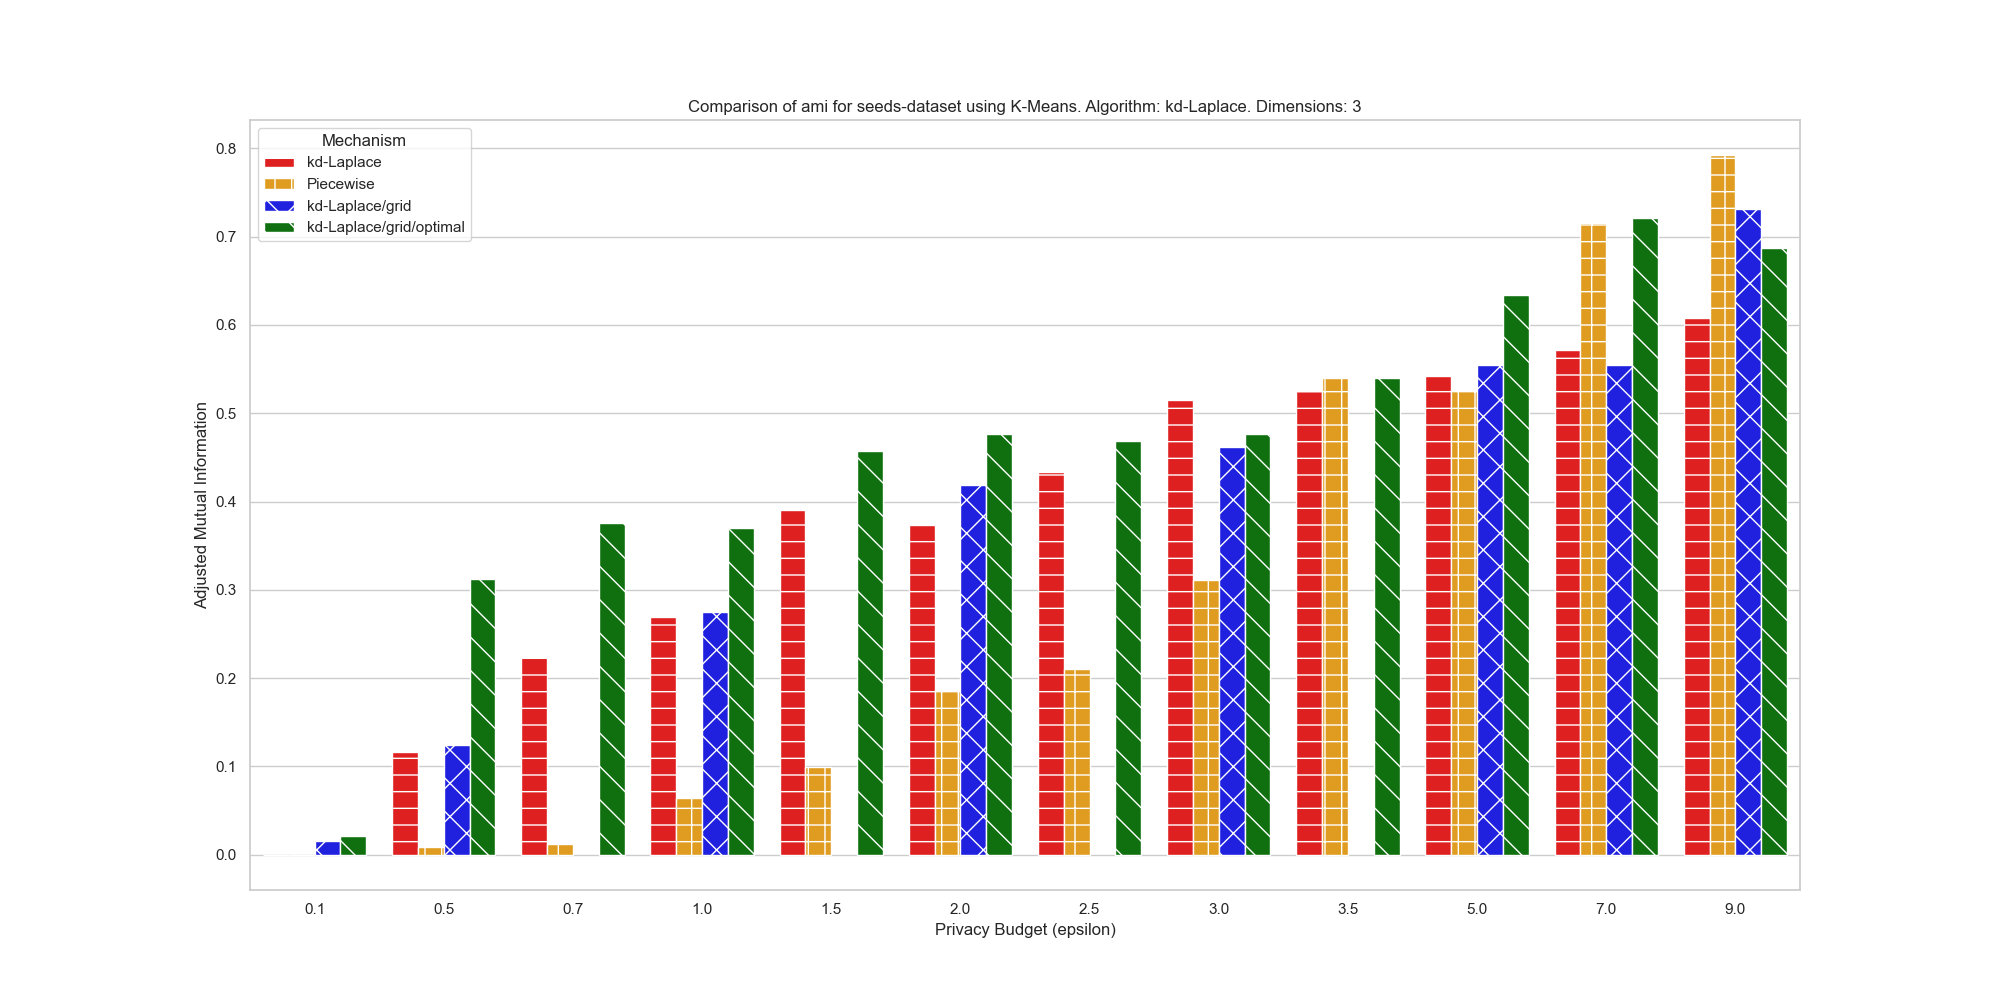
\includegraphics[width=\textwidth]{Results/RQ2/seeds-dataset/ami_seeds-dataset_comparison.png}
    \caption{Adjusted Mutual Information comparison for the 3-dimensional seeds-dataset}
    \label{fig:ami_seeds-dataset_comparison_3d}
\end{figure}
\todo[inline]{Add links to scilliouette plots and other plots}

\subsection{Privacy}
\begin{figure}[H]
    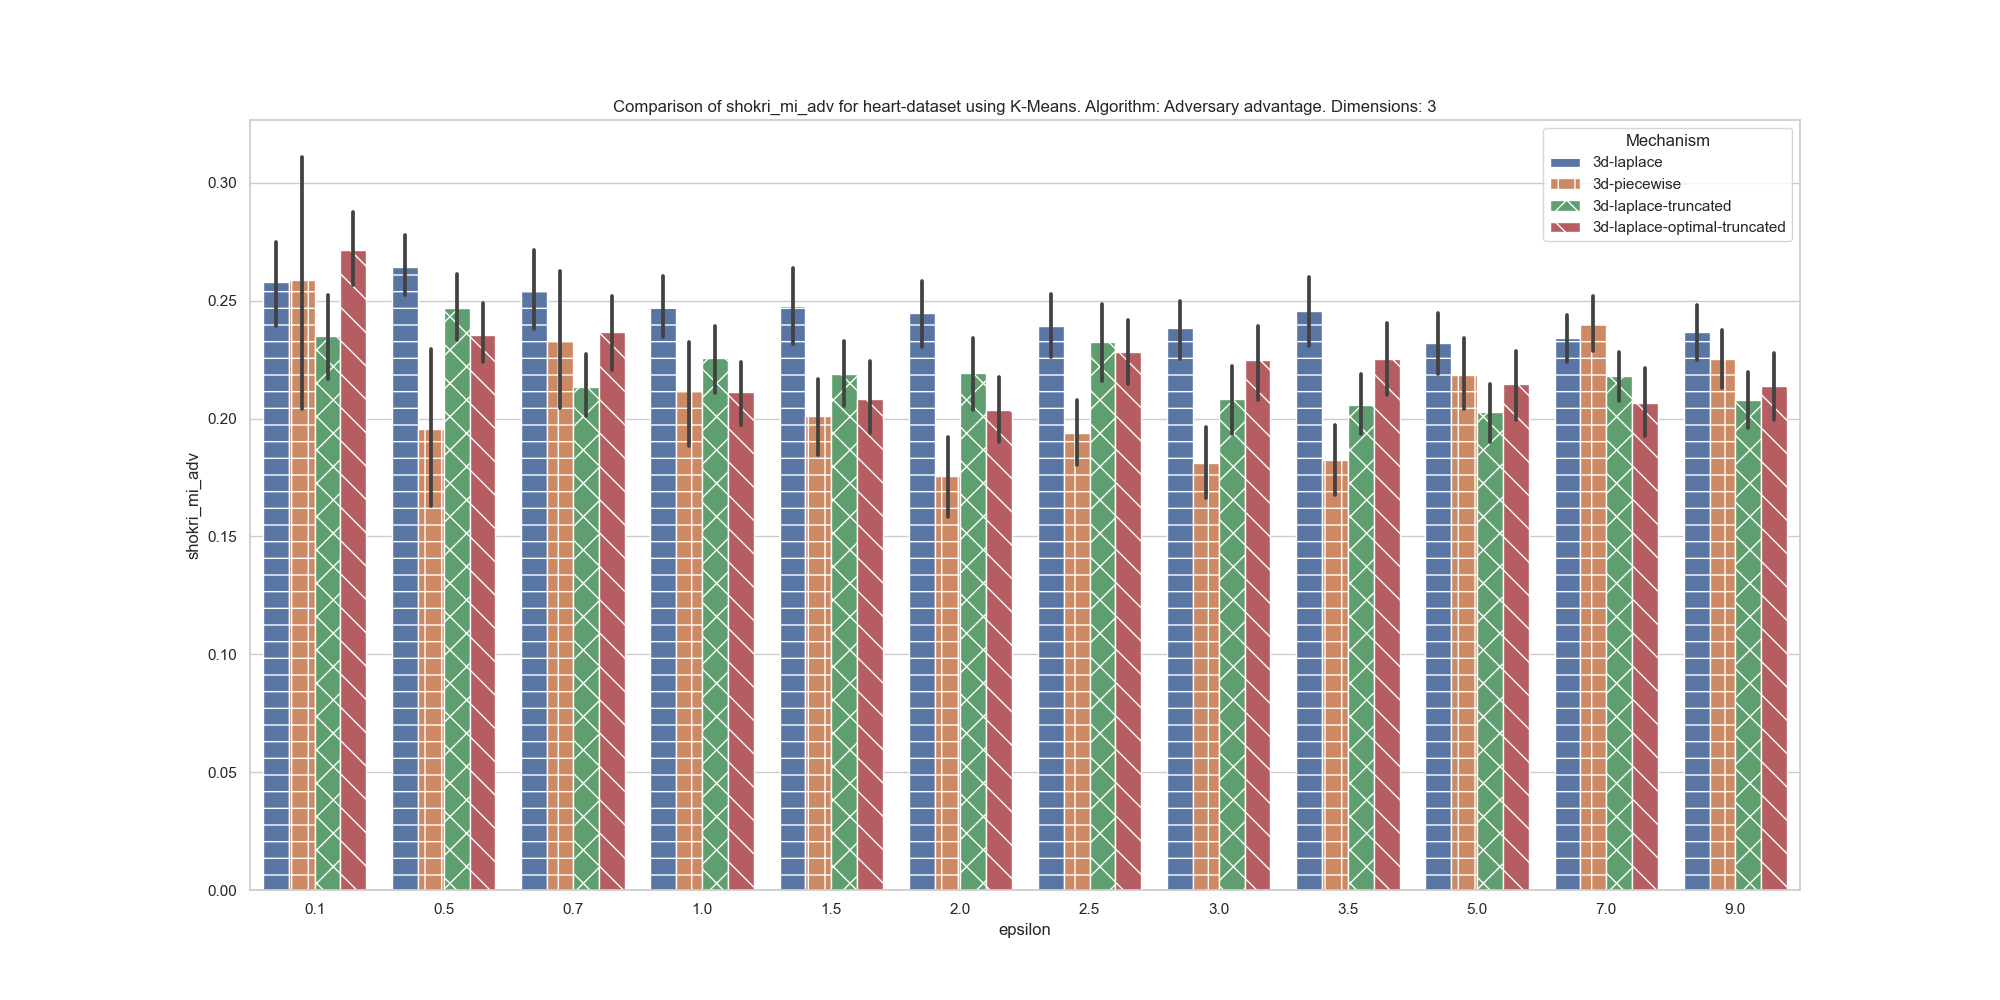
\includegraphics[width=\textwidth]{Results/RQ2/heart-dataset/shokri_mi_adv_heart-dataset_comparison.png}
    \caption{Skokri et al. privacy comparison for the 3-dimensional heart-dataset.}
    \label{fig:privacy_heart-dataset_comparison_3d}
\end{figure}
\begin{figure}[H]
    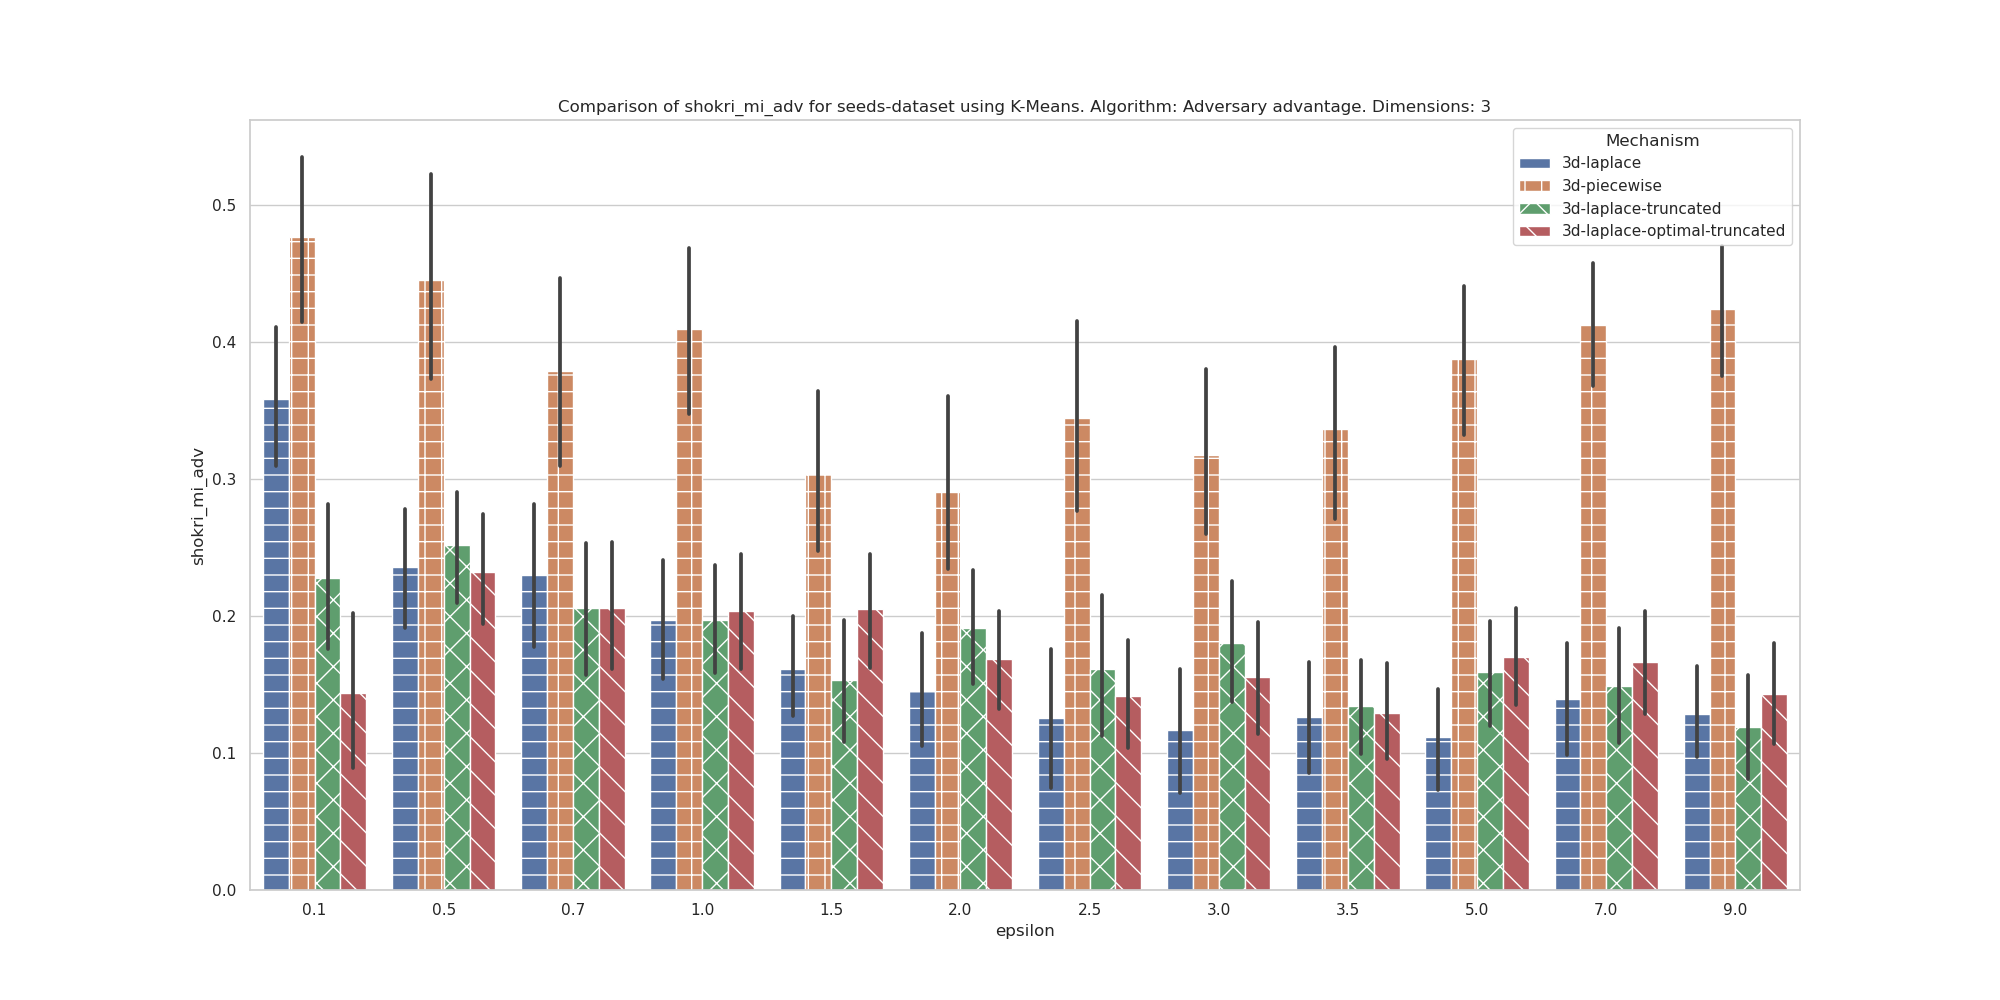
\includegraphics[width=\textwidth]{Results/RQ2/seeds-dataset/shokri_mi_adv_seeds-dataset_comparison.png}
    \caption{ROC-curve for privacy per privacy mechanism for 3-dimensional seeds-dataset.}
    \label{fig:privacy_seeds-dataset_comparison_3d}
\end{figure}
\begin{figure}[H]
    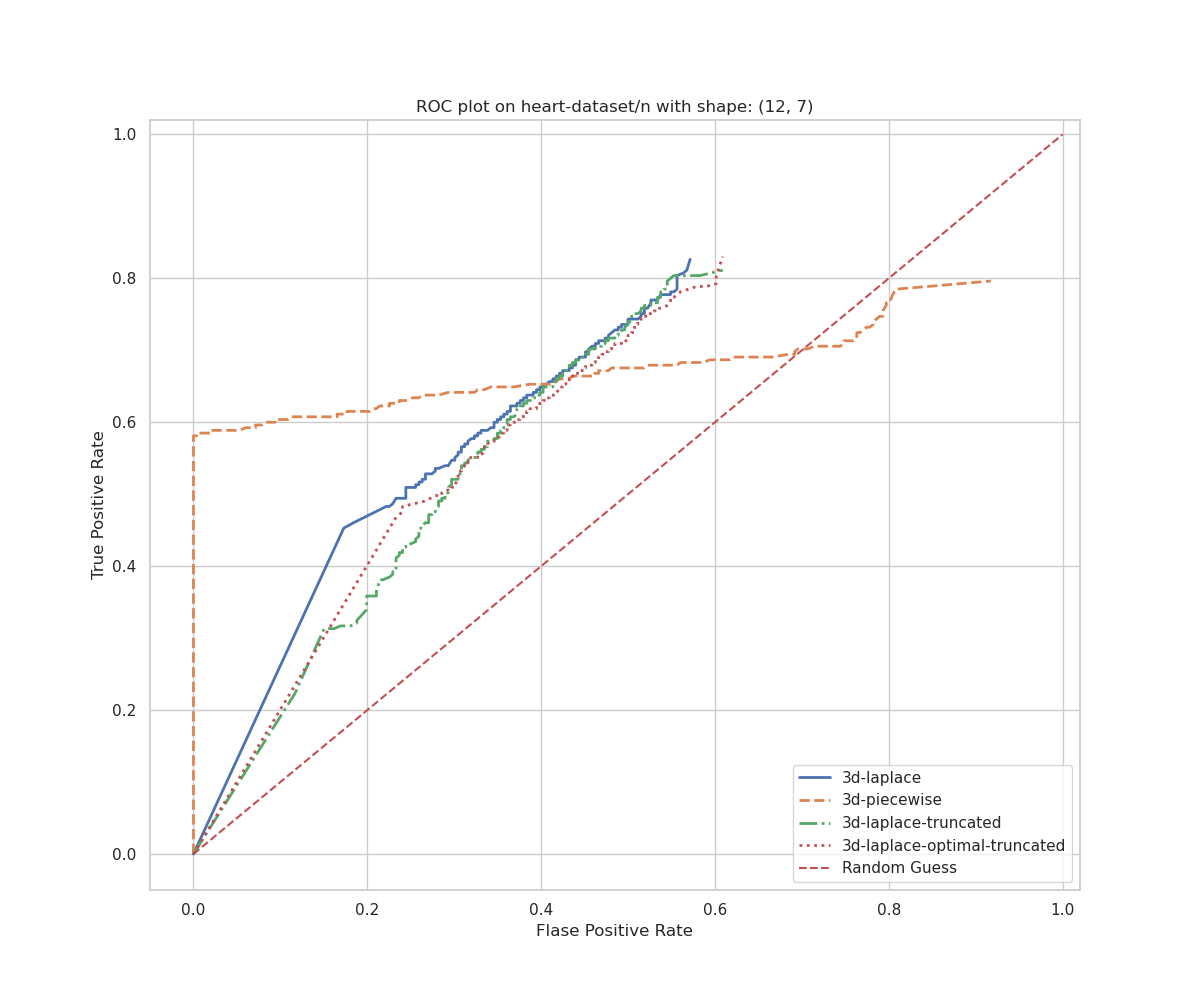
\includegraphics[width=0.8\textwidth]{Results/RQ2/heart-dataset/roc_plot.png}
    \caption{ROC-curve for privacy per privacy mechanism for 3-dimensional heart-dataset.}
    \label{fig:privacy_heart-dataset_comparison_3d_roc_plot}
\end{figure}

\begin{figure}[H]
    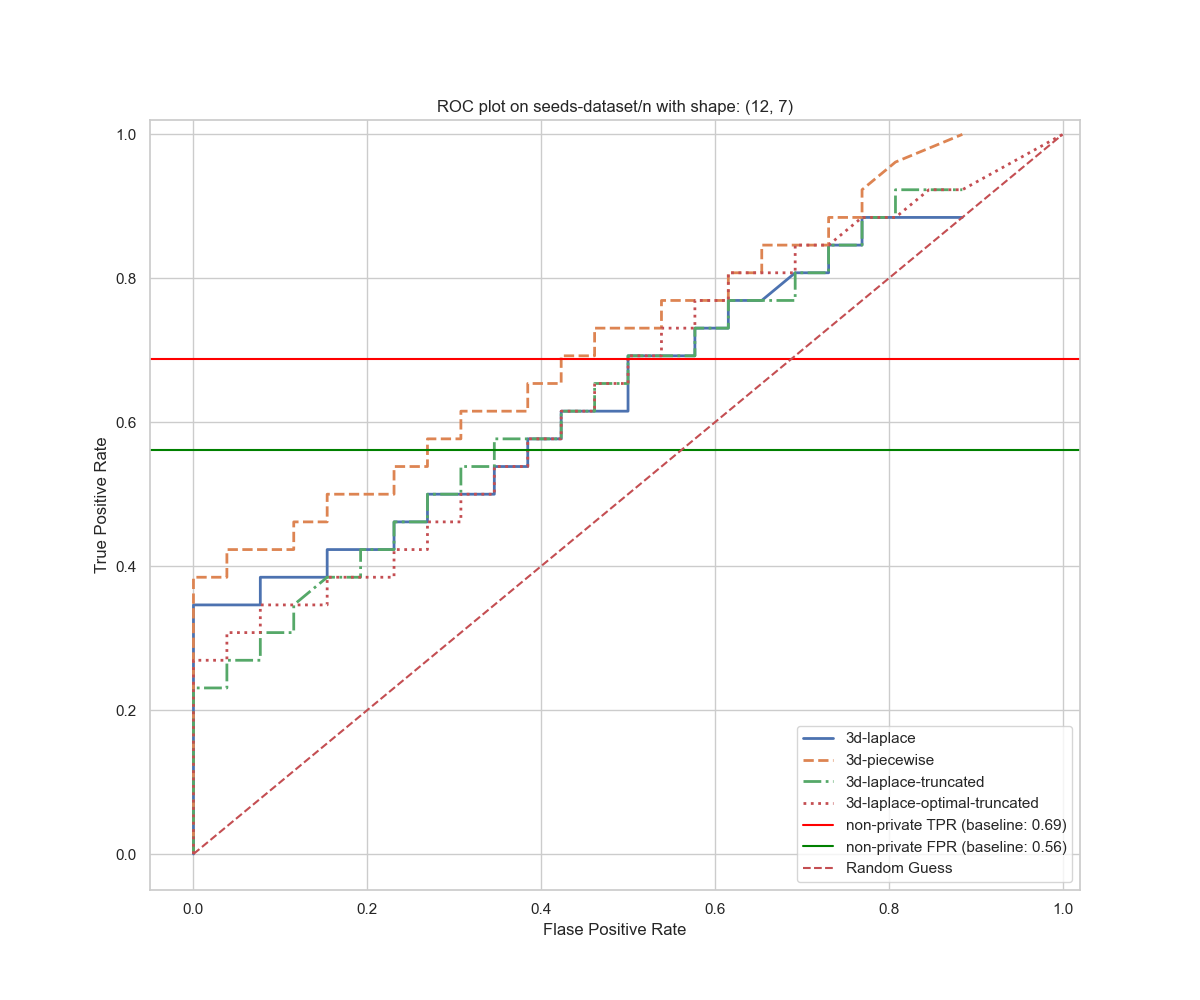
\includegraphics[width=0.8\textwidth]{Results/RQ2/seeds-dataset/roc_plot.png}
    \caption{ROC-curve for privacy per privacy mechanism for 3-dimensional seeds-dataset.}
    \label{fig:privacy_seeds-dataset_comparison_3d_roc_plot}
\end{figure}

\section{Research question 3}